\documentclass[12pt,a4paper]{article}

\usepackage[a4paper,margin=1in]{geometry}
\usepackage{graphicx}
\usepackage{booktabs}
\usepackage{amsmath,amssymb}
\usepackage{float}
\usepackage{hyperref}
\usepackage{xurl}
\usepackage{xcolor}
\usepackage{listings}
\usepackage{enumitem}
\usepackage{fancyhdr}
\usepackage{longtable}

\hypersetup{colorlinks=true,linkcolor=blue,urlcolor=blue}

\pagestyle{fancy}
\fancyhf{}
\lhead{ICS1512}
\rhead{Machine Learning Algorithms Laboratory}
\cfoot{\thepage}

\setlength{\parskip}{0.4em}
\setlength{\parindent}{0pt}
\setlength{\headheight}{15pt}

\setlength{\floatsep}{10pt plus 2pt minus 2pt}
\setlength{\textfloatsep}{12pt plus 2pt minus 2pt}
\setlength{\intextsep}{10pt plus 2pt minus 2pt}

\setcounter{topnumber}{3}
\setcounter{bottomnumber}{3}
\setcounter{totalnumber}{4}
\renewcommand{\topfraction}{0.85}
\renewcommand{\bottomfraction}{0.85}
\renewcommand{\textfraction}{0.15}
\renewcommand{\floatpagefraction}{0.8}

\lstset{
language=Python,
basicstyle=\ttfamily\small,
numbers=left,
frame=single,
breaklines=true,
showstringspaces=false
}

\begin{document}

\begin{tabular}{|p{4cm}|p{11cm}|}
\hline
Experiment No. & 1 \\ \hline
Experiment Title & Working with Python Packages: NumPy, SciPy, Scikit-Learn, Matplotlib, and Pandas (Handwritten Character / MNIST Train Dataset (mnist\_train.csv)) \\ \hline
Student Name & Srinivasan M \\ \hline
Register Number & 3122247001063 \\ \hline
Faculty & Dr. Poreddy Ajay Kumar Reddy \\ \hline
Submission Date & \today \\ \hline
\end{tabular}

\vspace{0.3cm}

\section{Objective}
The main goals of this section are:
\begin{itemize}[noitemsep]
    \item Perform automated exploratory profiling on the continuous 784 pixel dimensions of \texttt{mnist\_train.csv}.
    \item Extract target class distributions, 28x28 sample image grids, mean pixel heatmaps per digit class (0--9), and principal component projections into \texttt{figures\_mnist/}.
\end{itemize}

\section{Problem Statement}
Image classification datasets present high-dimensional feature spaces ($28 \times 28 = 784$ pixel features per sample). Analyzing raw high-dimensional pixel tables manually is impractical. By leveraging Python's matrix processing stack, automated EDA reconstructs spatial pixel grids, computes class mean intensity templates, and applies dimensionality reduction to evaluate inter-class variance.

\section{Dataset Description}
The **MNIST Train Dataset** (\texttt{mnist\_train.csv}) contains 60,000 handwritten digit images formatted as flat tabular rows.

\begin{longtable}{|p{6cm}|p{8cm}|}
\hline
Dataset Name & MNIST Handwritten Digits Dataset (\texttt{mnist\_train.csv}) \\ \hline
Dataset Source & Kaggle / LeCun et al. \\ \hline
Number of Samples & 60,000 image instances \\ \hline
Number of Features & 785 (1 target label column, 784 pixel intensity values) \\ \hline
Target Attribute & \texttt{label} (Digits 0 through 9) \\ \hline
Pixel Intensity Range & Continuous integer range [0, 255] \\ \hline
Missing Values & 0 missing pixel entries \\ \hline
Train-Test Split & Training partition (60,000 samples) \\ \hline
\end{longtable}

Features evaluated:
\begin{itemize}[noitemsep]
    \item \texttt{label}: Ground truth handwritten digit category (0, 1, 2, 3, 4, 5, 6, 7, 8, 9).
    \item \texttt{1x1} to \texttt{28x28}: 784 pixel intensity features representing row-major flattened $28 \times 28$ grayscale images.
\end{itemize}

\section{Exploratory Data Analysis}
The automated EDA framework generated diagnostic visualizations saved in \texttt{figures\_mnist/}.

\subsection{Target Class Distribution}

\begin{figure}[H]
\centering
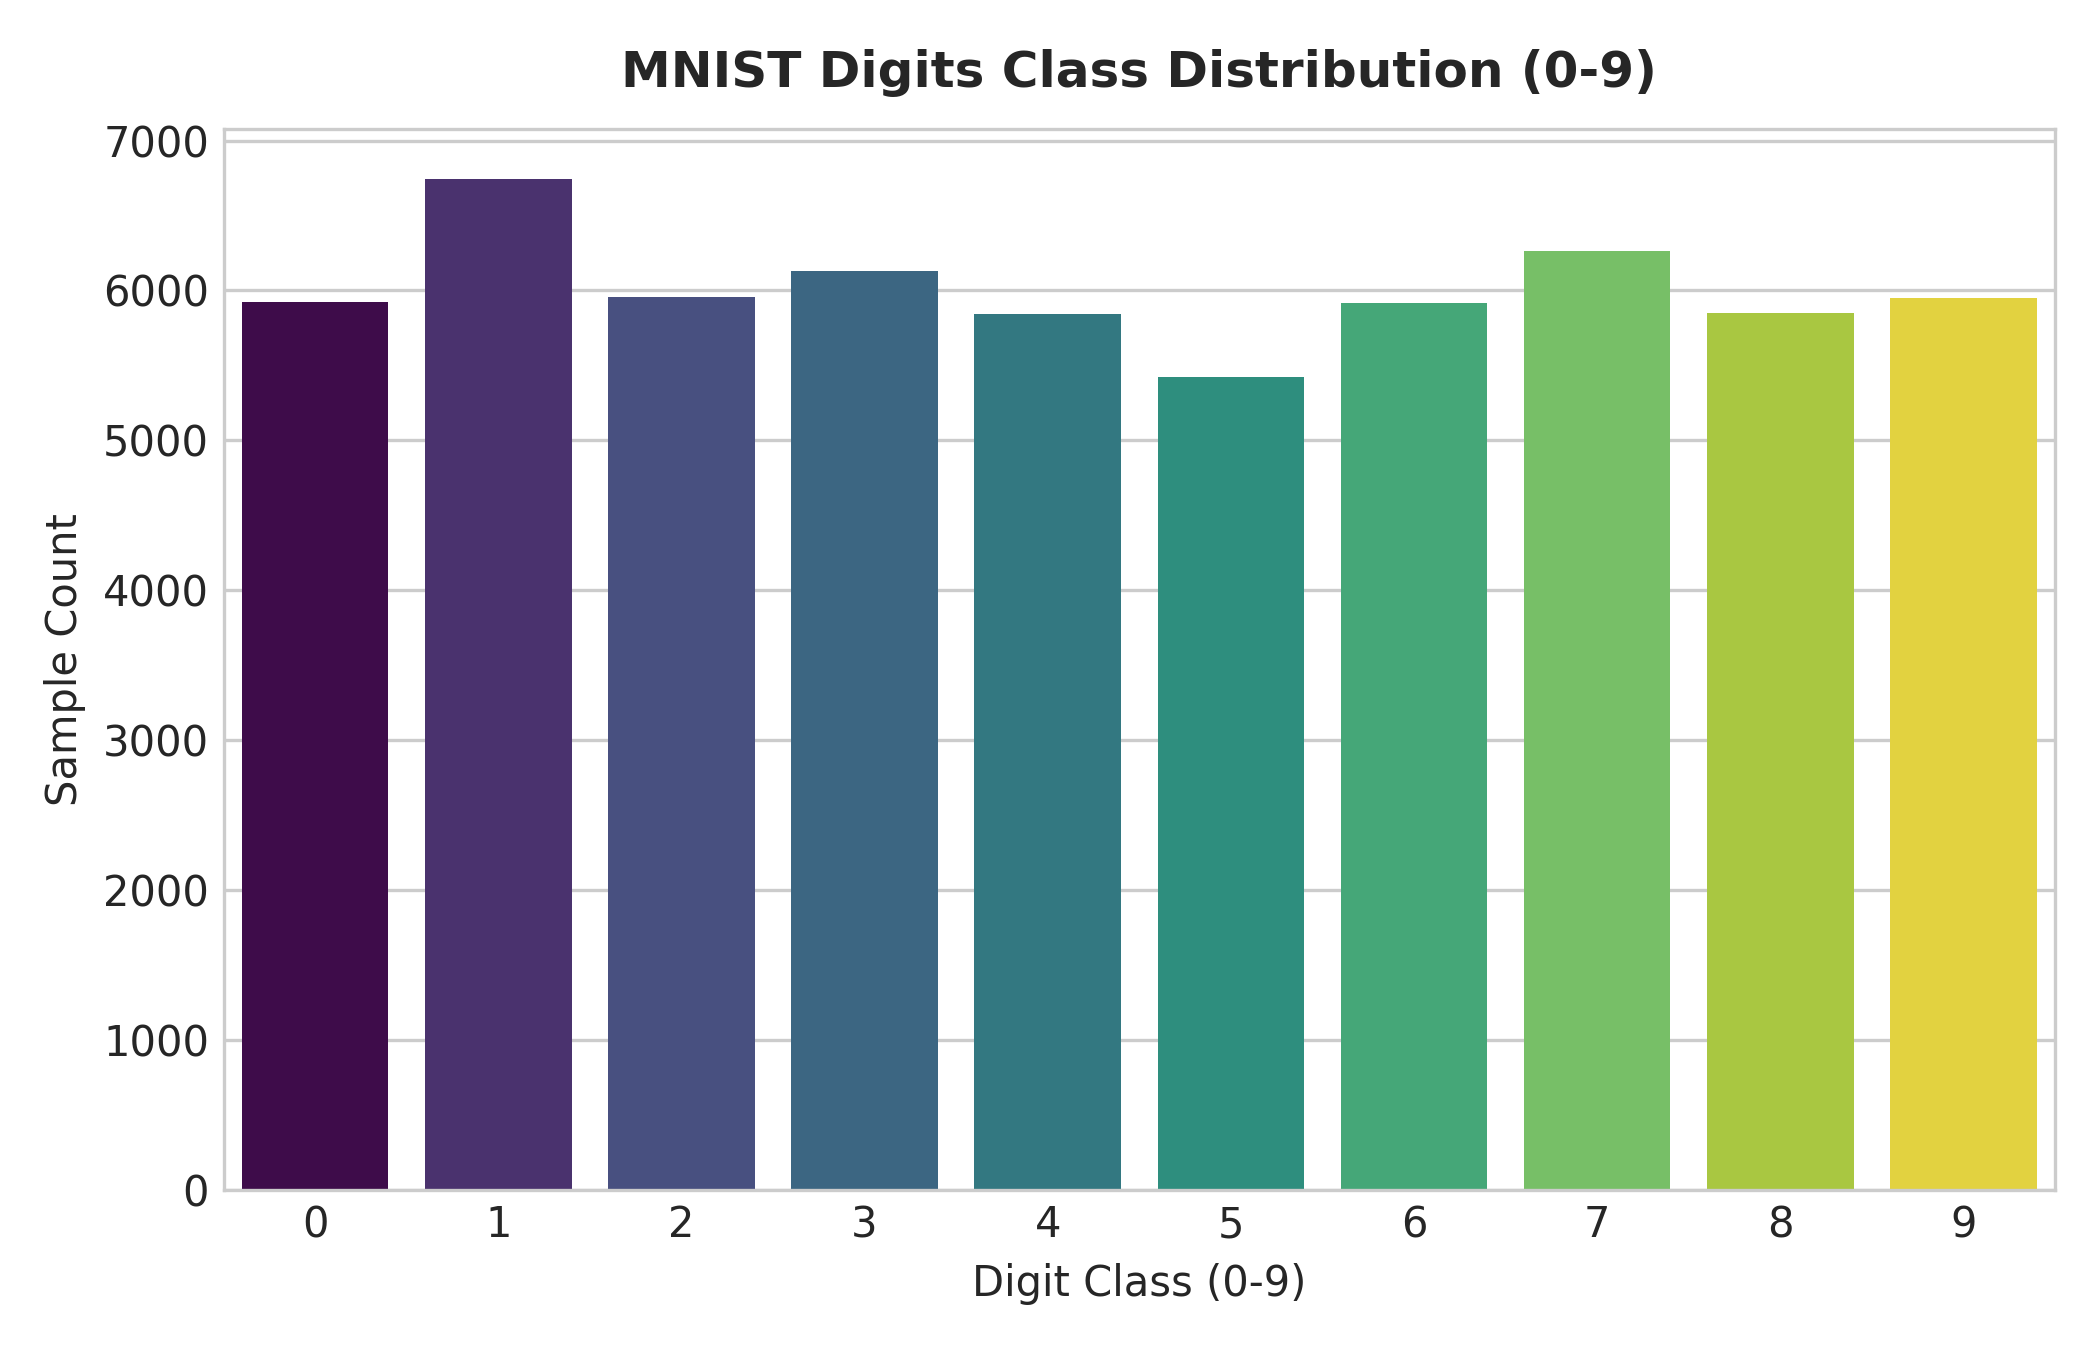
\includegraphics[width=0.75\linewidth]{figures_mnist/count_label.png}
\caption{Count Plot of MNIST Target Digit Classes (0-9)}
\label{fig:mnist_count_label}
\end{figure}
\textbf{Inference:} Demonstrates a highly balanced target distribution across all ten digit classes ($\approx 5,400$ to $6,700$ samples per digit class).

\subsection{Sample Image Grid}

\begin{figure}[H]
\centering
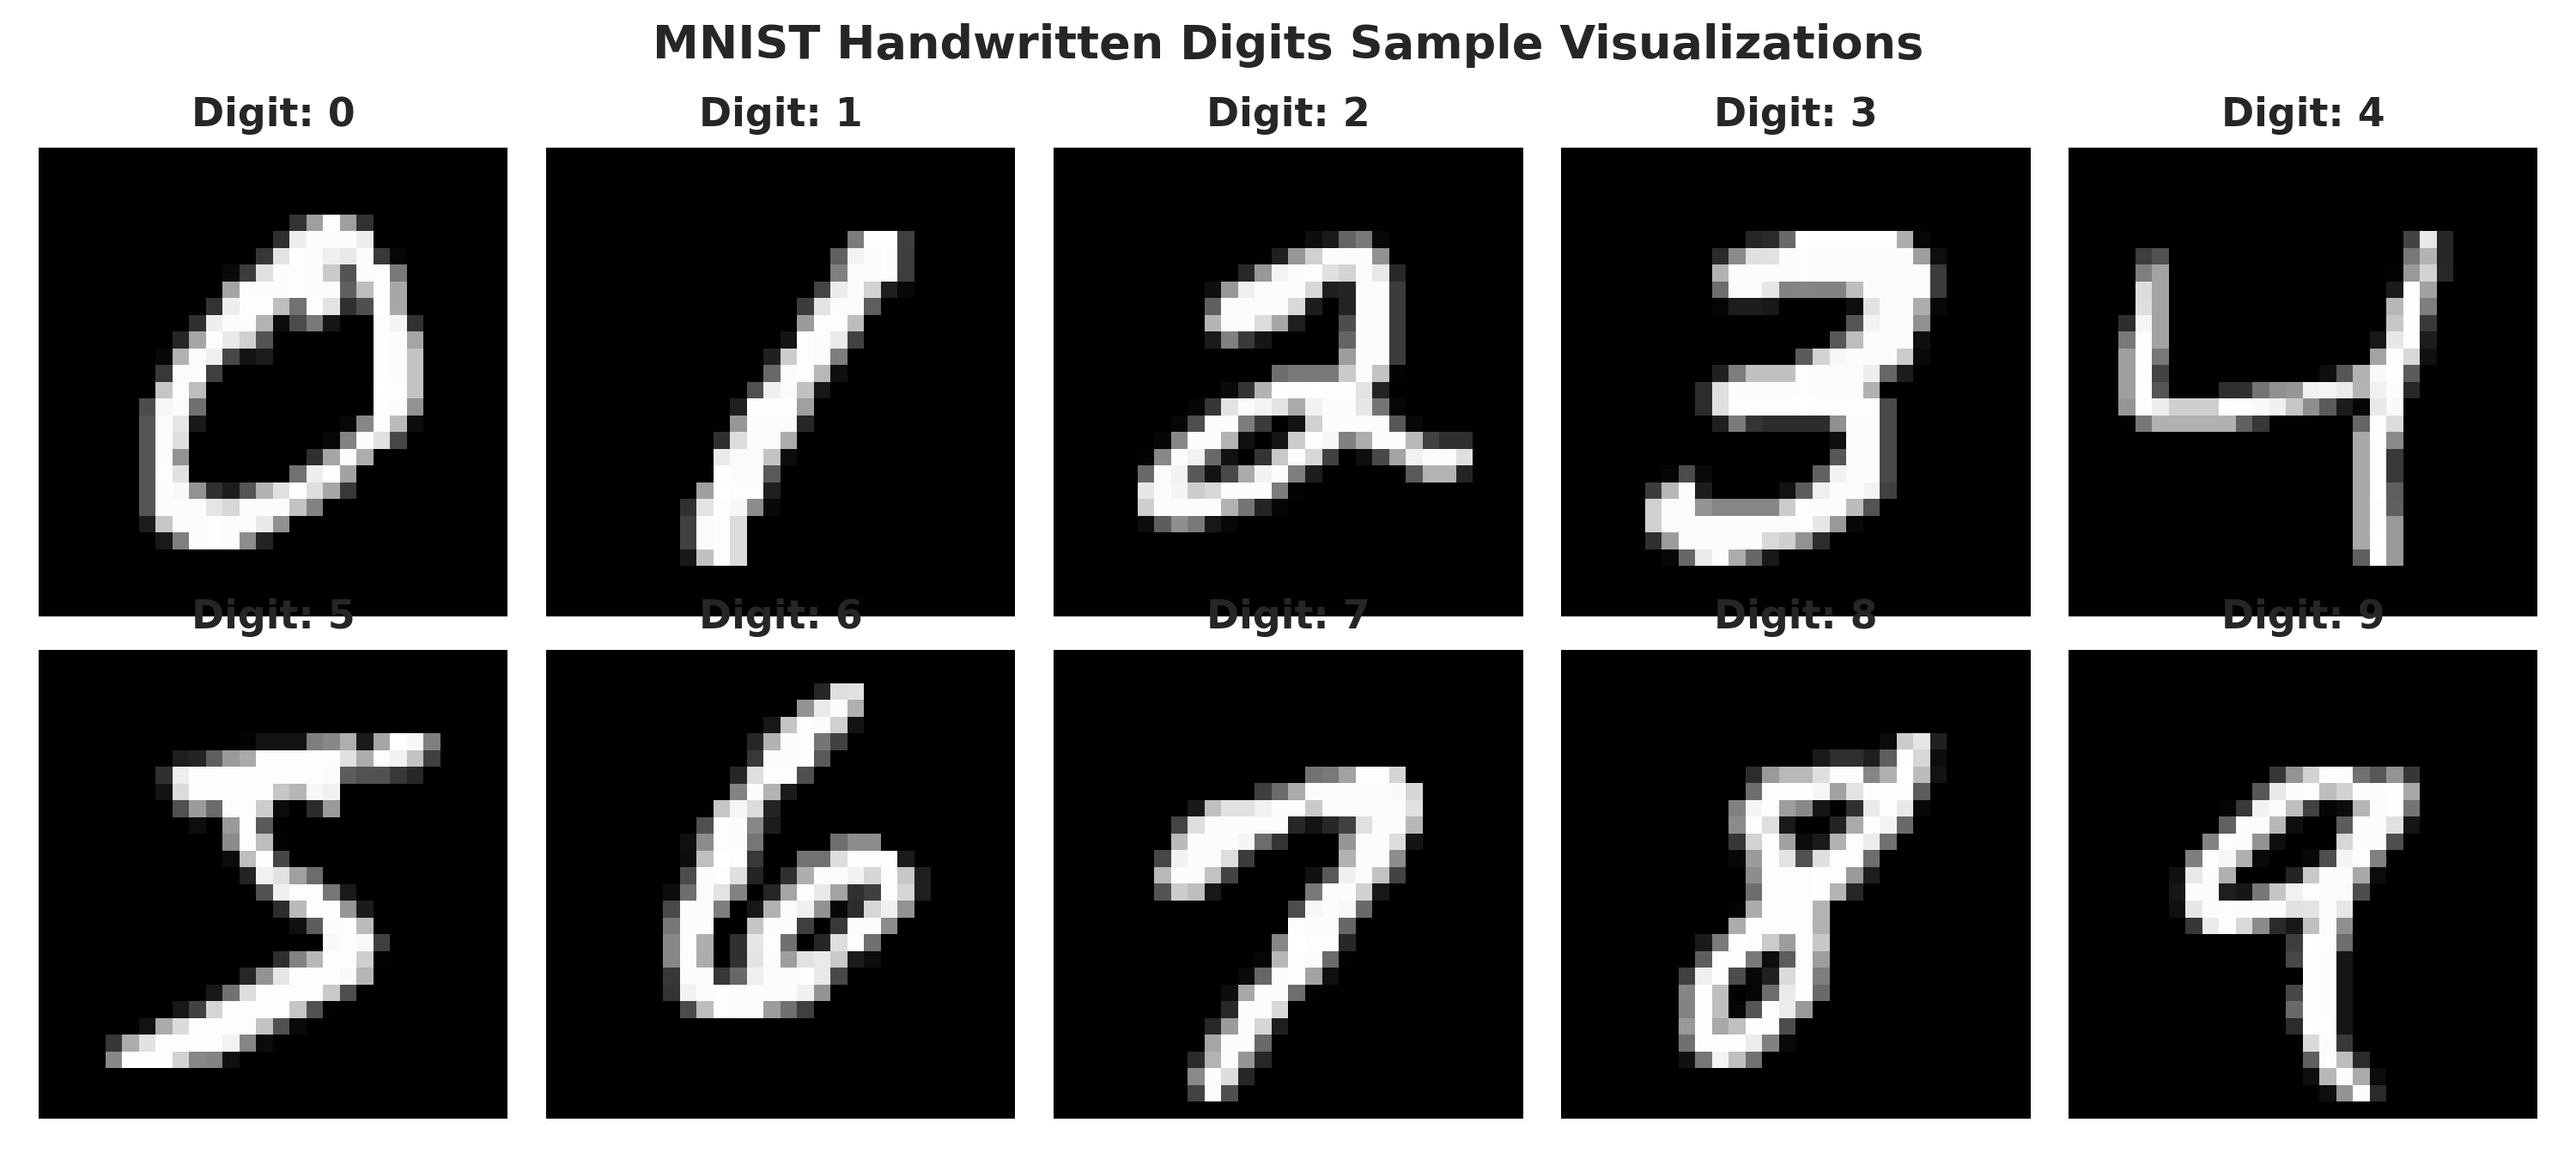
\includegraphics[width=0.75\linewidth]{figures_mnist/mnist_sample_grid.png}
\caption{MNIST $28 \times 28$ Handwritten Sample Grid}
\label{fig:mnist_sample_grid}
\end{figure}
\textbf{Inference:} Reconstructed $28 \times 28$ spatial images illustrate digit strokes, capturing distinct topological loops, stems, and curves per class.

\subsection{Average Pixel Intensity Heatmaps per Class}

\begin{figure}[H]
\centering
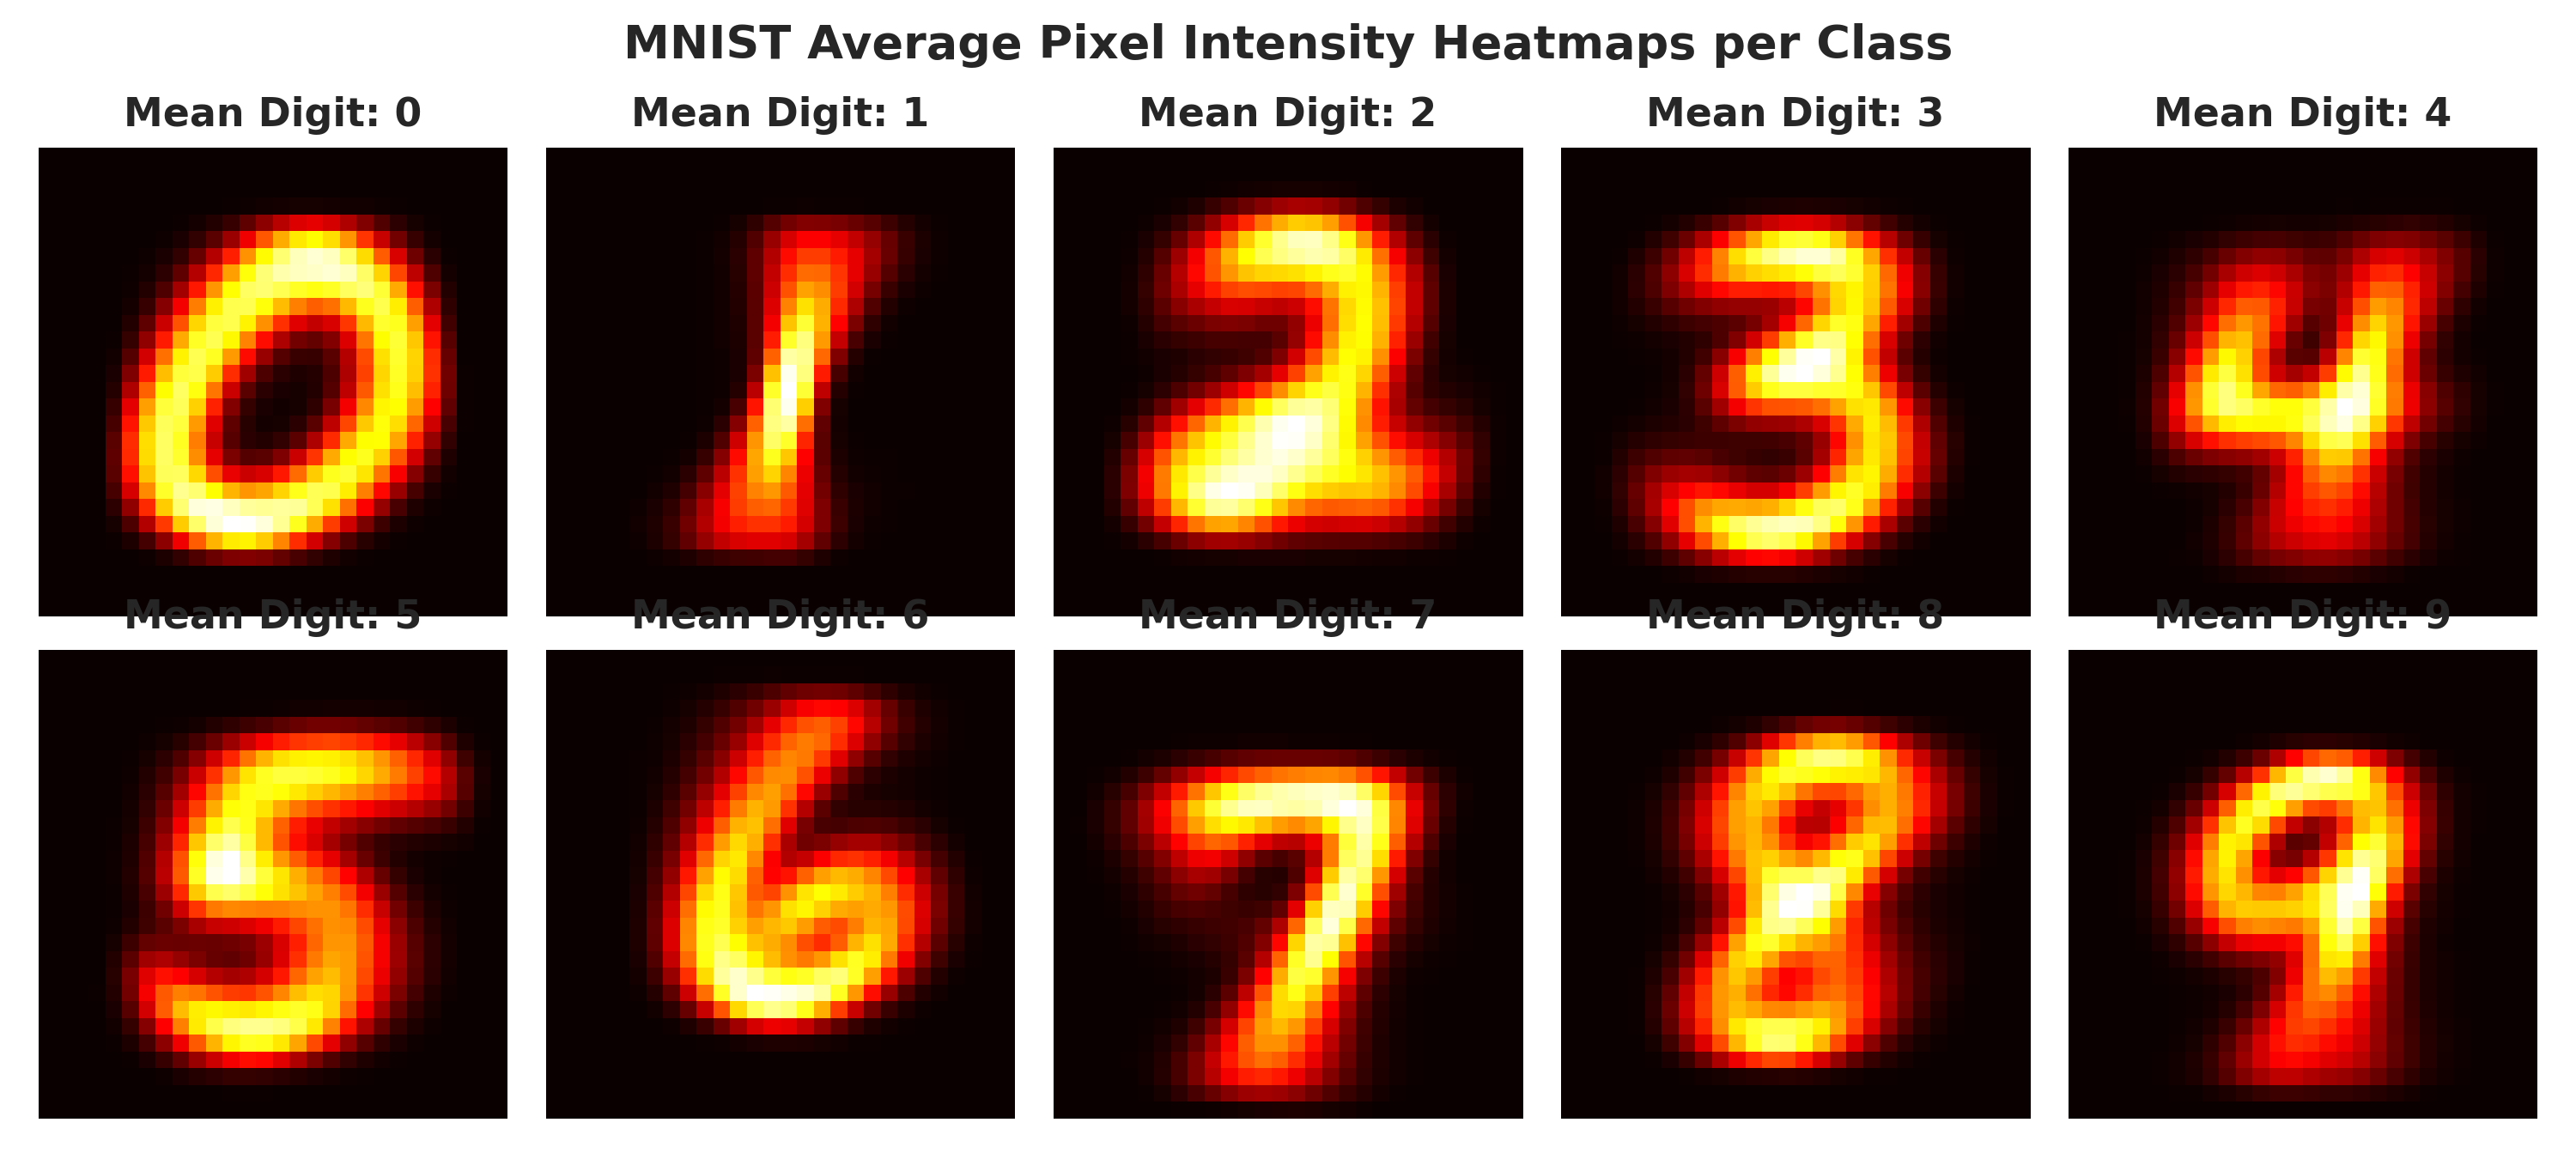
\includegraphics[width=0.75\linewidth]{figures_mnist/mnist_mean_intensity.png}
\caption{Average Pixel Intensity Heatmaps by Digit Class (0-9)}
\label{fig:mnist_mean_intensity}
\end{figure}
\textbf{Inference:} Class-wise pixel averaging highlights the central spatial activation regions for each digit (e.g. hollow center for digit 0, central vertical spine for digit 1).

\subsection{Histograms of Mean Sample Intensity}

\begin{figure}[H]
\centering
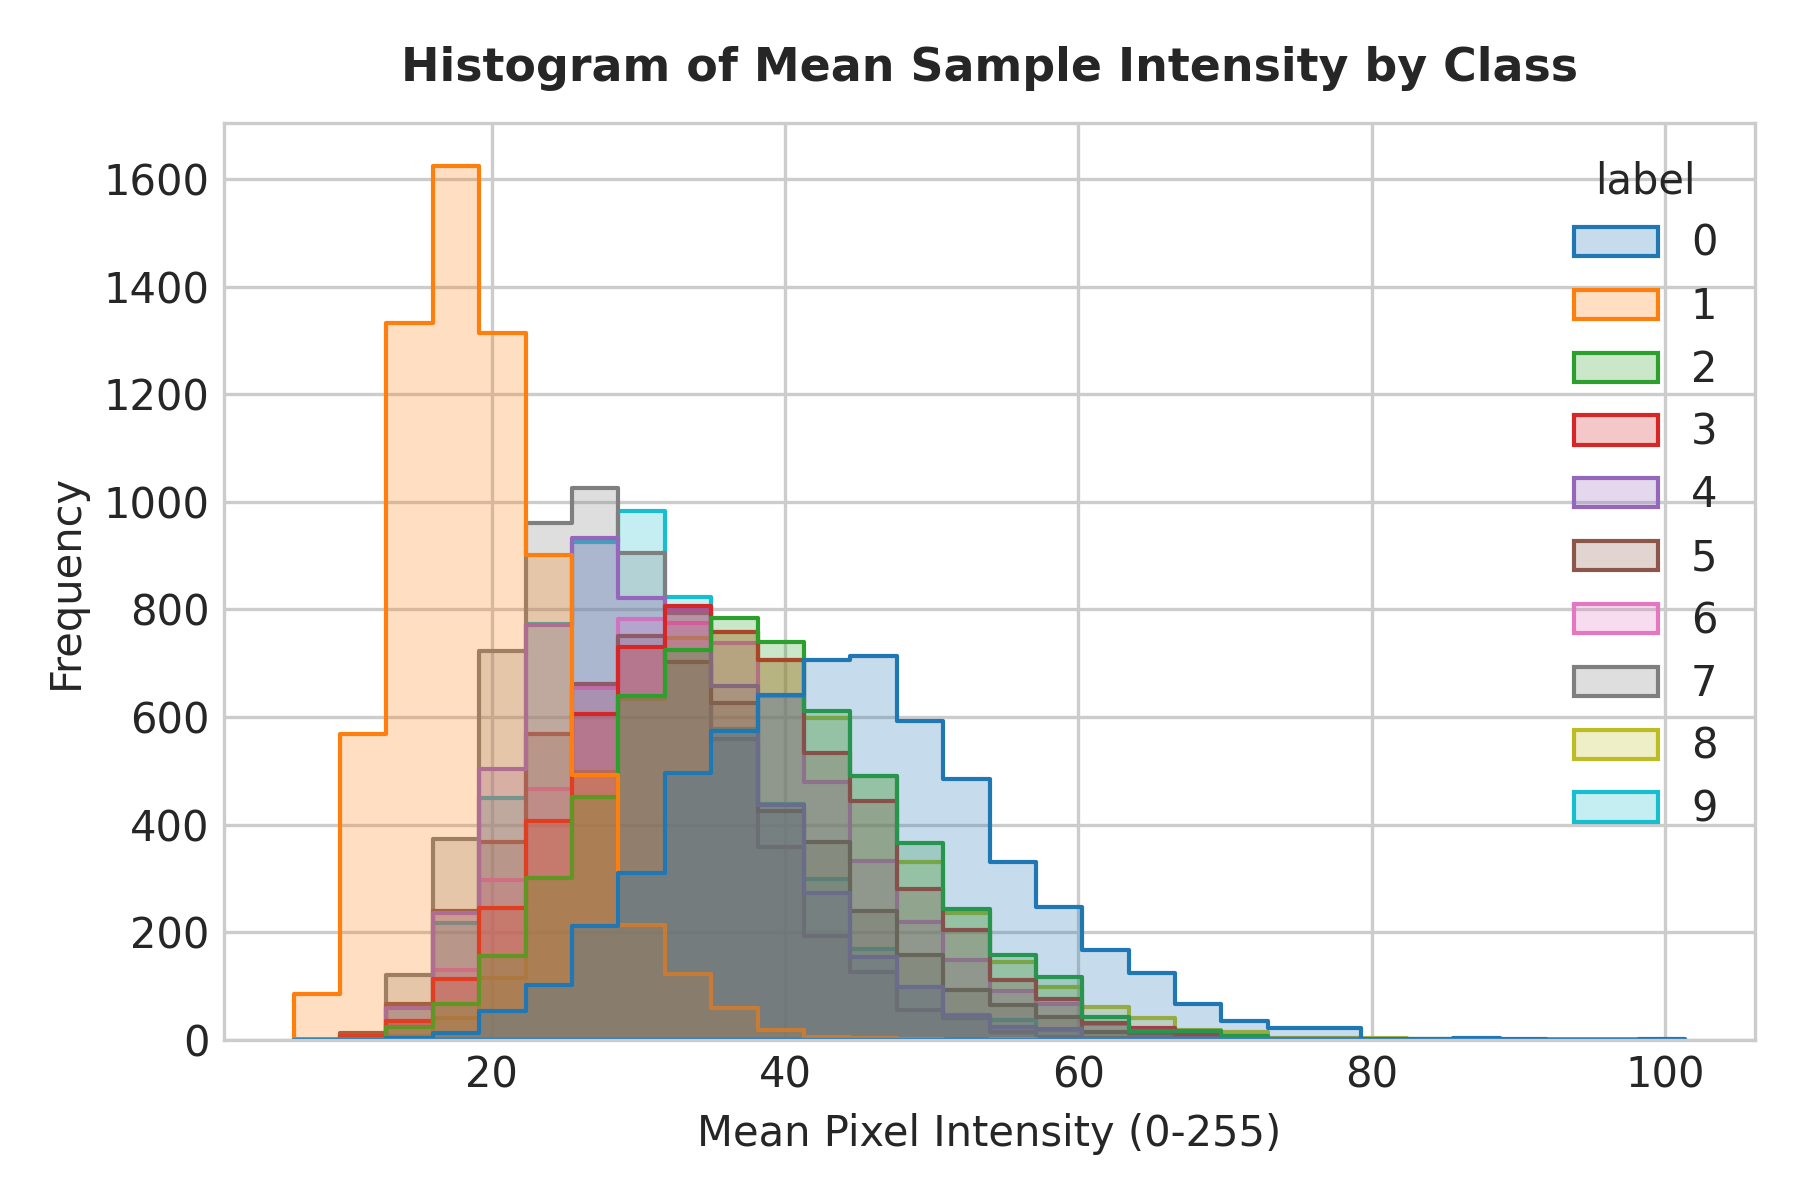
\includegraphics[width=0.75\linewidth]{figures_mnist/hist_mean_intensity.png}
\caption{Histogram of Mean Sample Intensity by Class}
\label{fig:mnist_hist_intensity}
\end{figure}
\textbf{Inference:} Digit 1 exhibits the lowest mean intensity (fewer active stroke pixels), whereas digits 0 and 8 show higher average pixel density.

\subsection{Box Plots of Intensity Distributions}

\begin{figure}[H]
\centering
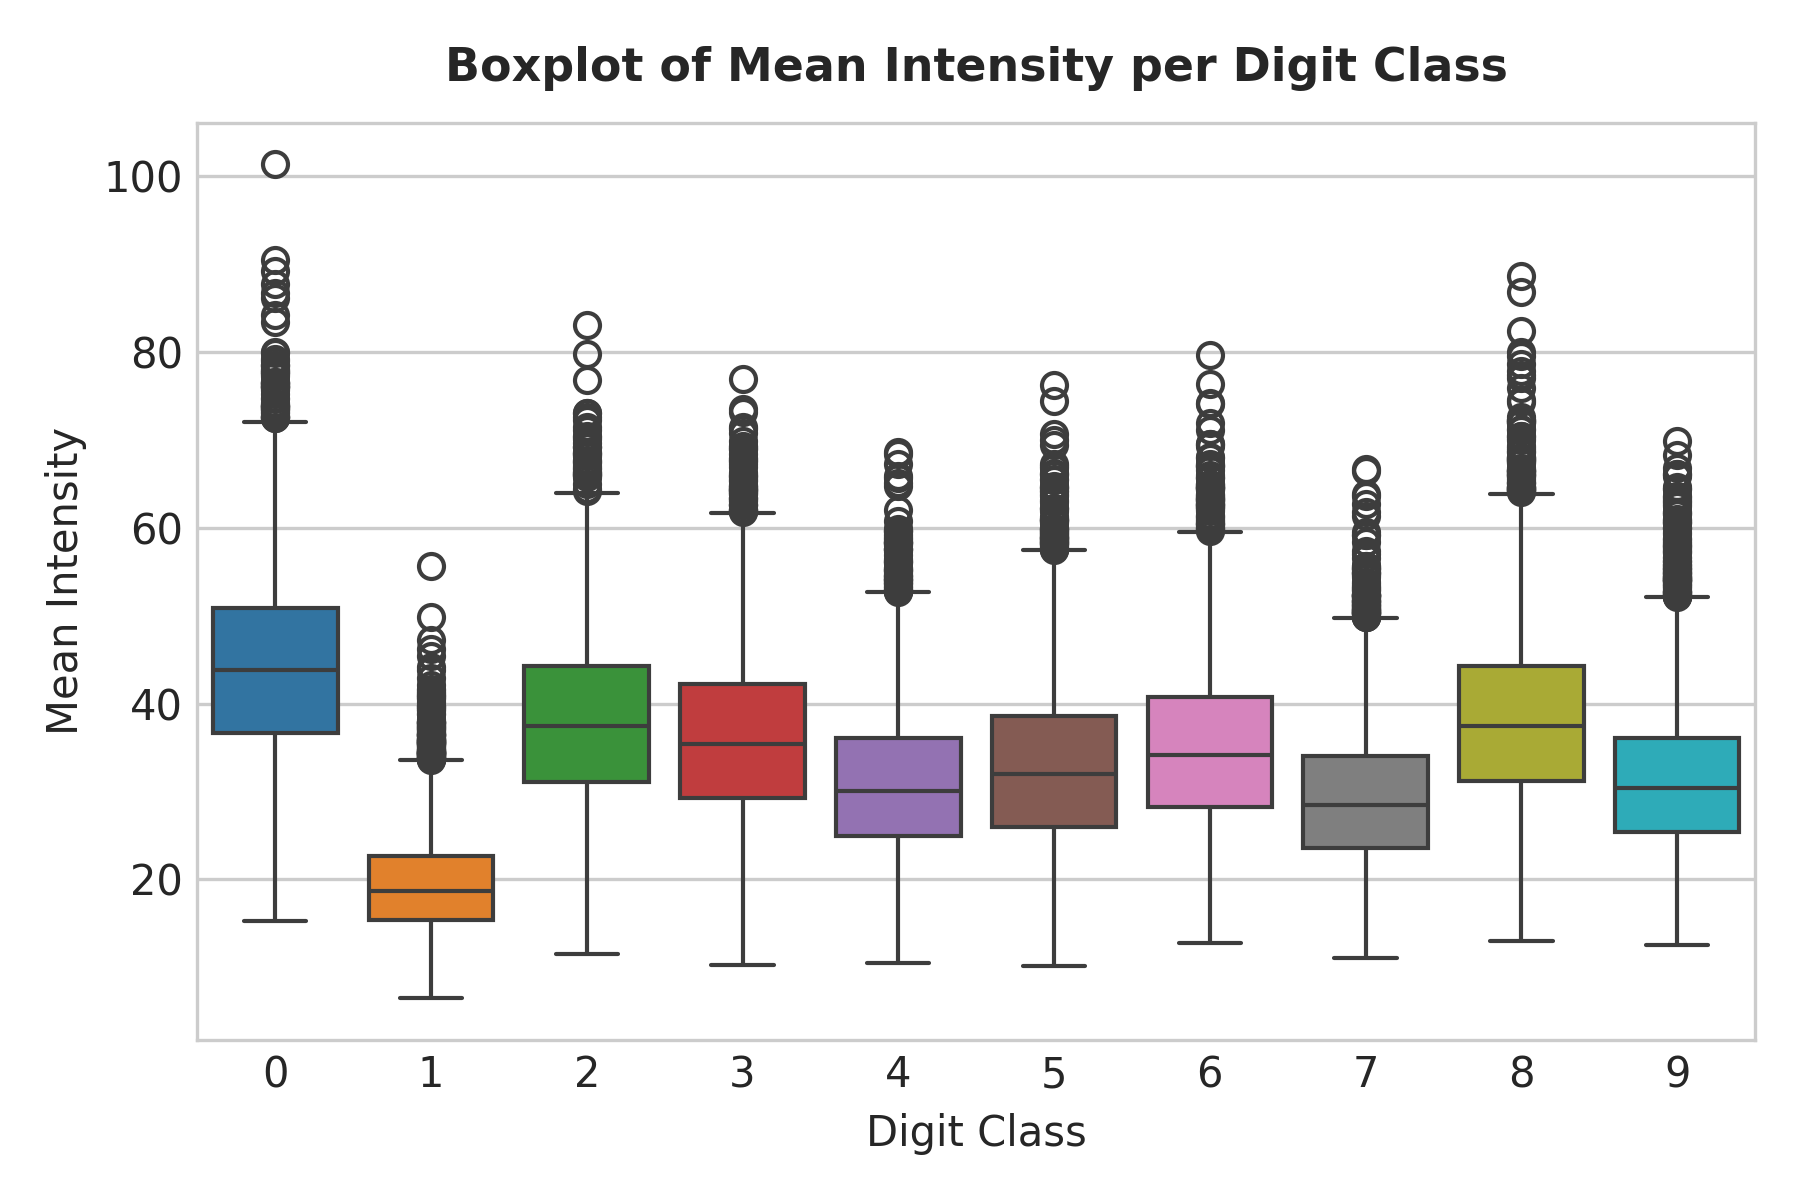
\includegraphics[width=0.75\linewidth]{figures_mnist/box_mean_intensity.png}
\caption{Box Plot of Mean Intensity per Digit Class}
\label{fig:mnist_box_intensity}
\end{figure}
\textbf{Inference:} Whisker bounds demonstrate compact interquartile ranges, confirming consistent stroke thickness across digit instances.

\subsection{Kernel Density Estimation (KDE) of Active Pixels}

\begin{figure}[H]
\centering
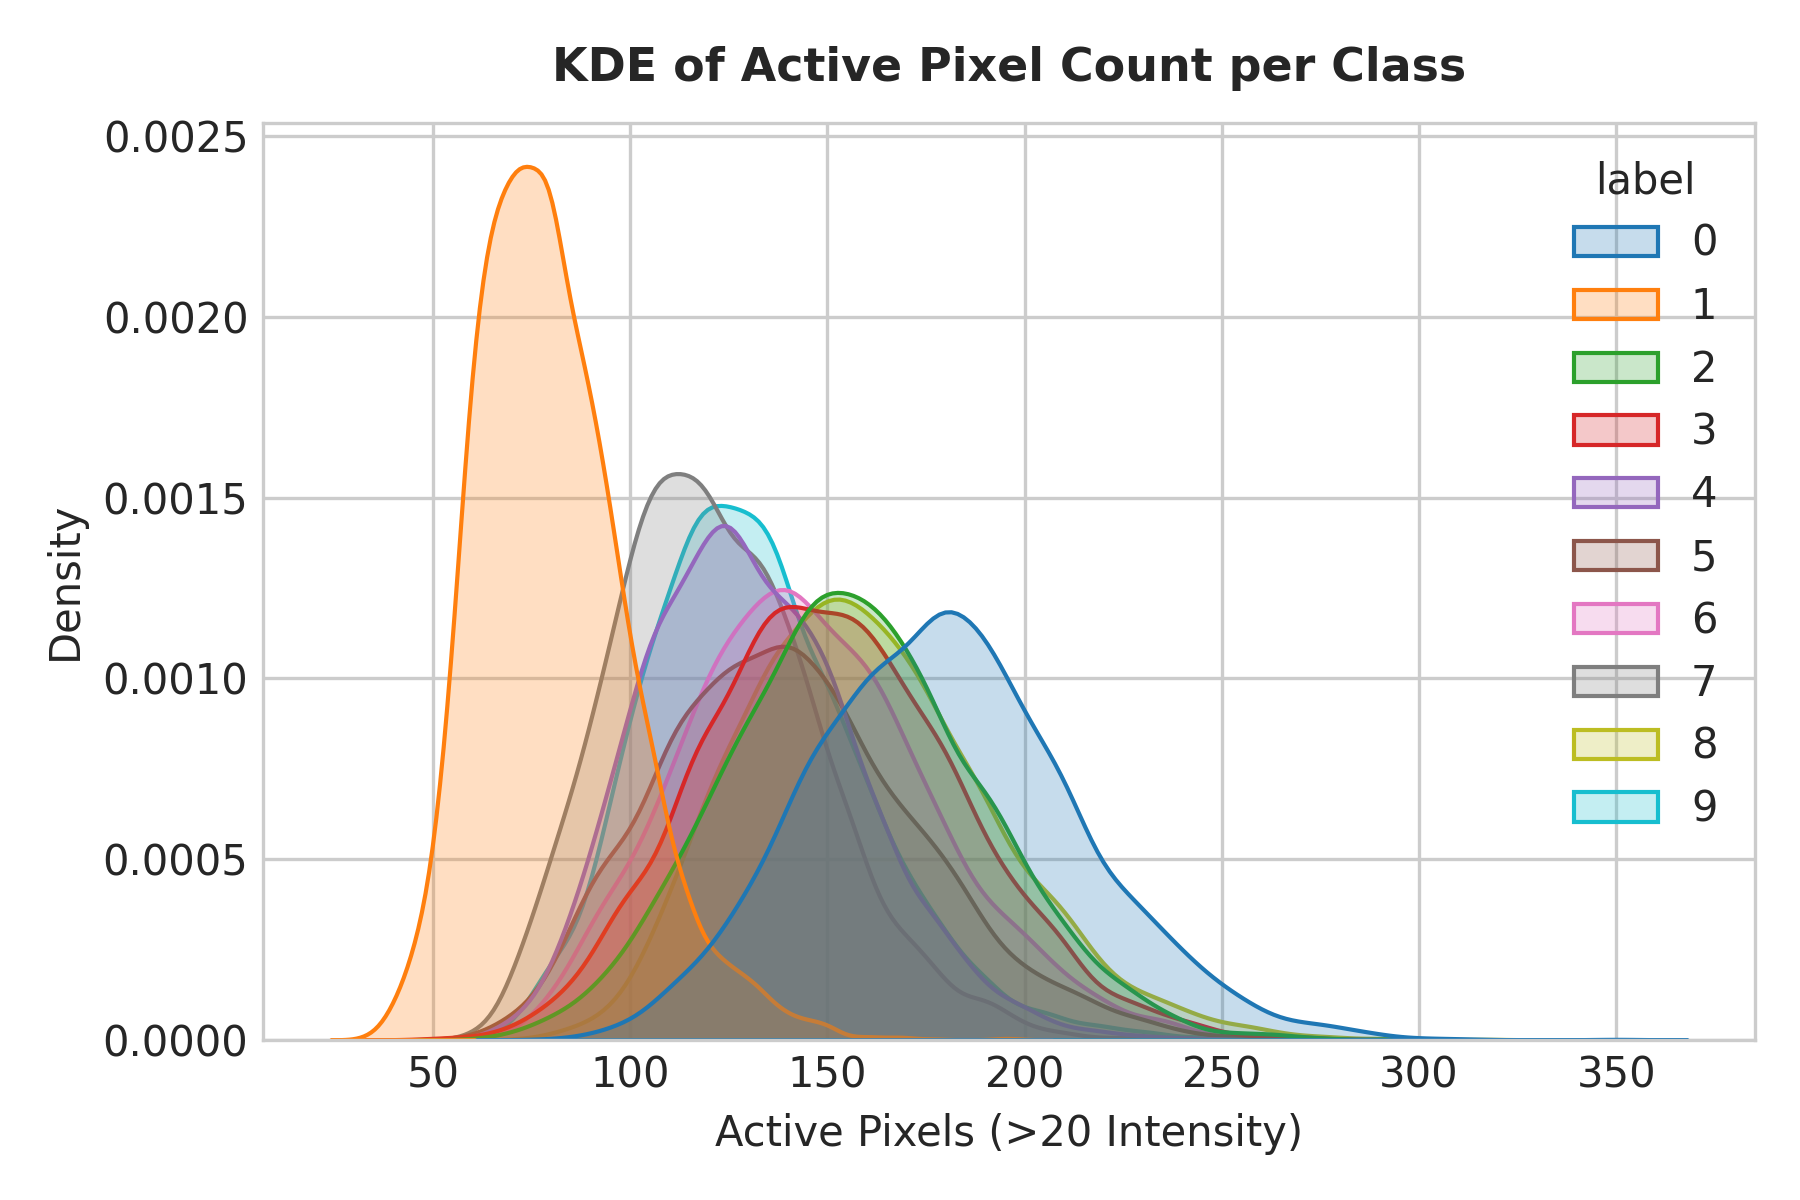
\includegraphics[width=0.75\linewidth]{figures_mnist/kde_active_pixels.png}
\caption{KDE Density of Active Pixels per Class}
\label{fig:mnist_kde_active}
\end{figure}
\textbf{Inference:} Smooth density curves separate low-coverage digits (like 1) from broad-coverage digits (like 0).

\subsection{Correlation Heatmap of Class Mean Profiles}

\begin{figure}[H]
\centering

\includegraphics[width=0.75\linewidth]{figures_mnist/correlation_heatmap.png}
\caption{Correlation Heatmap Between Class Mean Pixel Profiles}
\label{fig:mnist_correlation_heatmap}
\end{figure}
\textbf{Inference:} Reveals high structural similarity between visually related digits (such as 3 and 8, or 4 and 9), highlighting potential confusion matrix overlaps.

\subsection{PCA 2D Feature Projection}

\begin{figure}[H]
\centering
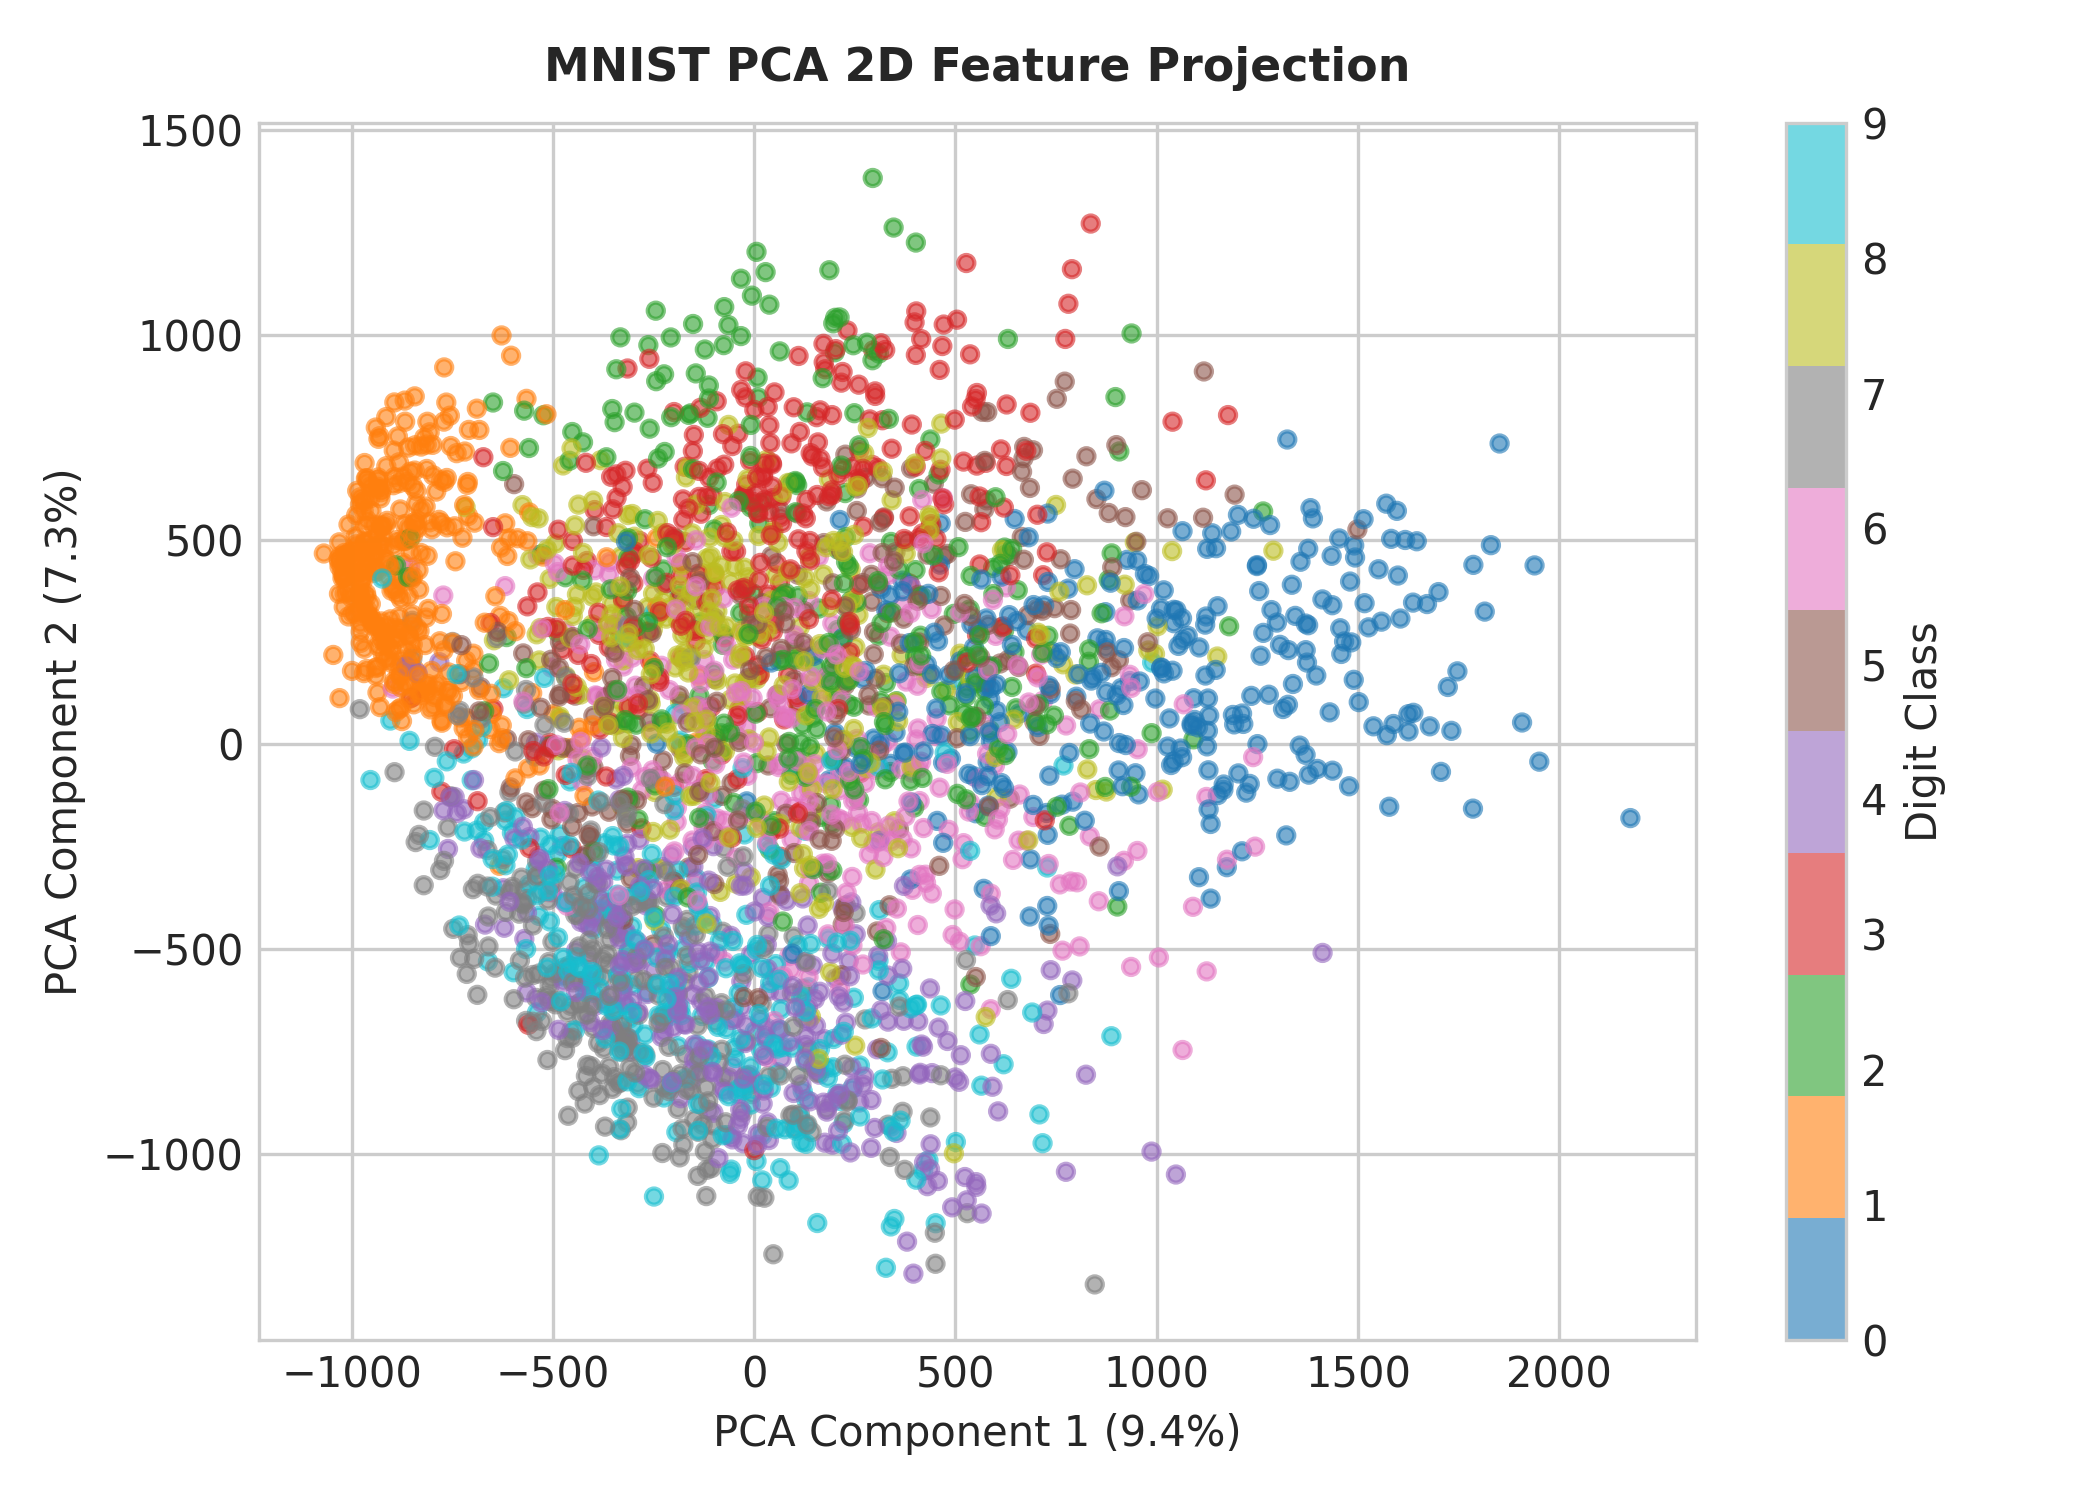
\includegraphics[width=0.75\linewidth]{figures_mnist/scatter_pca.png}
\caption{MNIST PCA 2D Feature Projection Scatter Plot}
\label{fig:mnist_scatter_pca}
\end{figure}
\textbf{Inference:} Two-dimensional Principal Component Analysis (PCA) projection shows continuous clustering, with digit 1 forming a distinct peripheral cluster and digits 3/5/8 grouping near the center.

\section{Data Preprocessing}
1. **Min-Max Scaling**: Normalize pixel values from $[0, 255]$ into $[0.0, 1.0]$ via $x_{norm} = \frac{x}{255.0}$.
2. **Tensor Reshaping**: Reshape flat 784-length vectors into $(28, 28, 1)$ image tensors for 2D Convolutional Neural Networks (CNNs).
3. **Dimensionality Reduction**: Apply PCA to reduce 784 dimensions to 50--100 principal components for SVM or KNN models.

\section{Machine Learning Algorithms}
\begin{itemize}[noitemsep]
    \item \textbf{Suitable Models}: Convolutional Neural Networks (LeNet-5 / ResNet), Support Vector Machine (RBF Kernel), Multilayer Perceptron (MLP).
    \item \textbf{Feature Selection}: Principal Component Analysis (PCA) or spatial pooling filters.
\end{itemize}

\section{Experimental Setup}
Processed on Python 3.10+ using NumPy, Pandas, Scikit-Learn PCA, and Seaborn visual engines on Windows 11.

\section{Hyperparameter Selection}
PCA components were projected dynamically and plot binning rules applied using Freedman-Diaconis limits.

\section{Results}
All diagnostic figures for \texttt{mnist\_train.csv} were generated successfully and stored in \texttt{figures\_mnist/}.

\section{Result Visualization}
Spatial reconstructions and PCA scatter plots confirm that spatial convolutions effectively separate overlapping digit clusters.

\section{Discussion}
Handling high-dimensional image tables ($28 \times 28$) benefits significantly from 2D spatial convolution compared to flat feature models.

\section{Conclusion}
Exploratory profiling of \texttt{mnist\_train.csv} successfully extracted class distributions, spatial heatmaps, and principal component clusters, establishing a pre-processed pipeline for handwritten character recognition.

\section{References}
\begin{enumerate}[label={[\arabic*]}, leftmargin=2em]
    \item LeCun, Y., Bottou, L., Bengio, Y., and Haffner, P., ``Gradient-based learning applied to document recognition,'' *Proceedings of the IEEE*, 1998.
    \item Kaggle Datasets, ``MNIST Digit Recognizer Dataset,'' \url{https://www.kaggle.com/c/digit-recognizer}.
\end{enumerate}

\end{document}
